\documentclass{beamer}
% September 2016 
% Author: Dr. Rachid Hourizi and Dr. Michael Wright 
% Department of Computer Science, University of Bath
\usepackage{listings}
\usepackage{tikz}

\usetheme{Boadilla} 
\lstset{language=C}

\begin{document}

\AtBeginSection[]{
  \begin{frame}
  \vfill
  \centering
  \begin{beamercolorbox}[sep=8pt,center,shadow=true,rounded=true]{title}
    \usebeamerfont{title}\insertsectionhead\par%
  \end{beamercolorbox}
  \vfill
  \end{frame}
}

\title{CM 10227/50258: UNIX 1}
\author{Dr. Rachid Hourizi and Dr. Michael Wright }
\date{\today}
\frame{\titlepage}
\frame{ 

\frametitle{Table of Contents}
\tableofcontents{}}

\section{Introduction to UNIX}

\begin{frame}
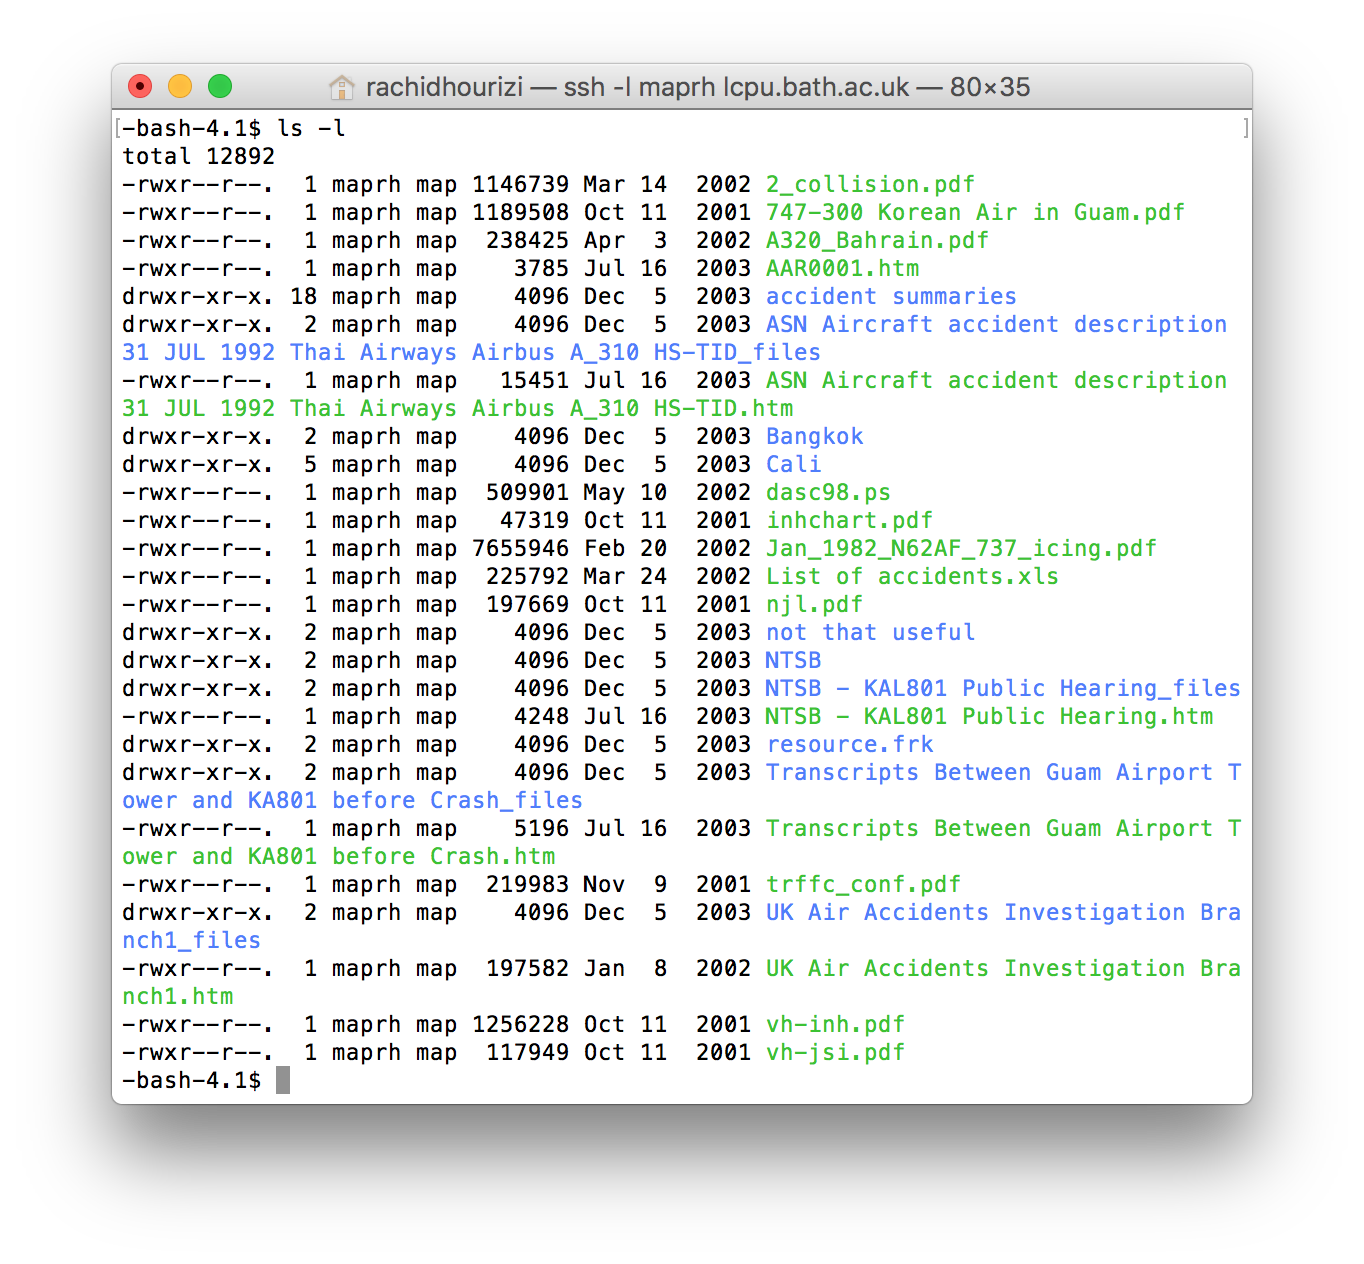
\includegraphics[height=9.5cm,keepaspectratio]{terminal}
\end{frame}

\subsection{The Command Line}
\begin{frame}\frametitle{Why Command-line?}
\begin{itemize}
\item Most modern tools have a graphical user interface (GUI)
\begin{itemize}
    \item Because they're easier to use
\end{itemize}
\item But command-line user interfaces (CLUIs) still have their place
\begin{itemize}
    \item Easier (faster) to build new CLUI tools
\begin{itemize}
          \item Building a GUI takes time
          \item Building a good GUI takes a lot of time
\end{itemize}
    \item Easier to see and understand what the computer is doing on your behalf
\begin{itemize}
          \item Which is part of what this course is about
\end{itemize}
    \item Most important: it's easier to combine CLUI tools than GUI tools
\begin{itemize}
          \item Small tools, combined in many ways, can be very powerful
\end{itemize}
\end{itemize}
\end{itemize}
\end{frame}

\subsection{The Shell}
\begin{frame}\frametitle{The Shell}
The most important command-line tool is the command shell (often just called “the shell”)
\begin{itemize}
    \item Manages a user's interactions with the operating system by:
\begin{itemize}
          \item Reading commands from the keyboard
          \item Figuring out what programs the user wants to run
          \item Running those programs
          \item Displaying their output on the screen
\end{itemize}
    \item Looks (and works) like an interactive terminal circa 1980
\end{itemize}
\end{frame}

\begin{frame}\frametitle{The Terminal}
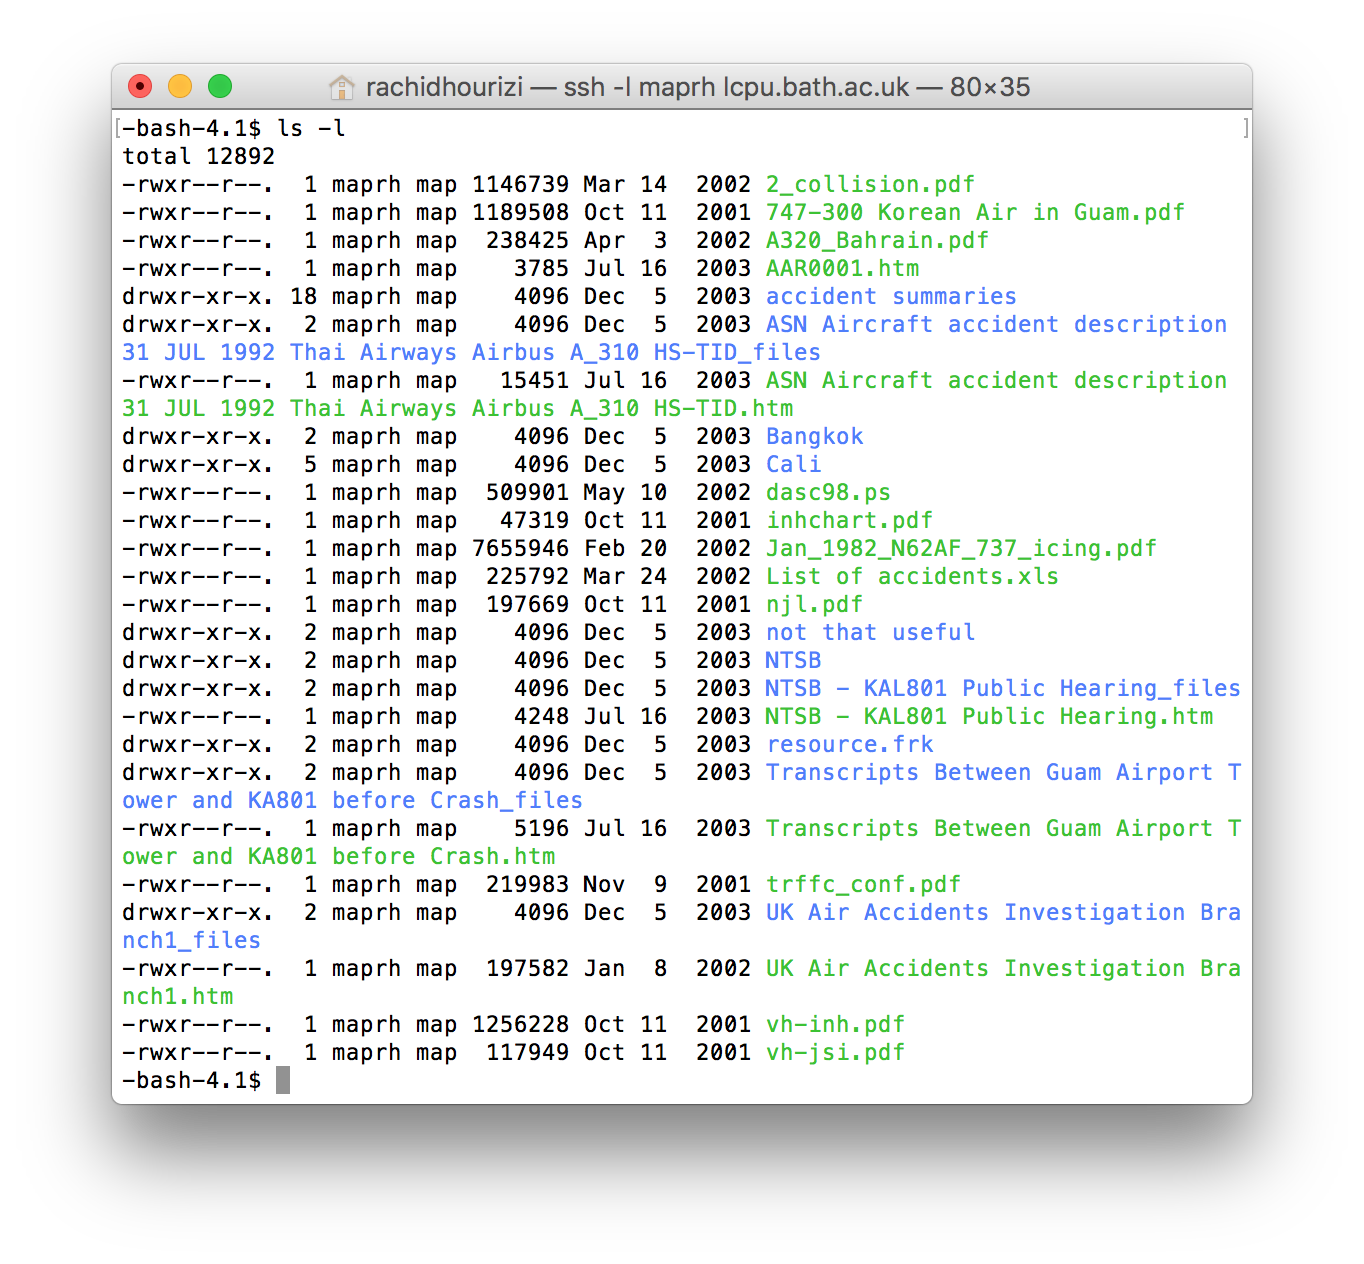
\includegraphics[height=9.5cm,keepaspectratio]{terminal}
\end{frame}

\begin{frame}\frametitle{The Shell vs. the Operation System}
\begin{itemize}
\item The shell is just one program among many
\begin{itemize}
    \item Many different ones have been written
    \item \textbf{sh} was the first for Unix
	\begin{itemize}
          \item Most others extend its capabilities in various ways
          \item Which means that it's the lowest common denominator you can always rely on
	\end{itemize}
    \item We will use \textbf{bash} (the Bourne again shell)
\begin{itemize}
          \item Available just about everywhere
          \item Even on Windows (thanks to Cygwin)
\end{itemize}
\end{itemize}
\end{itemize}
\end{frame}

\begin{frame}
\textbf{Aside: Cygwin}
\begin{itemize}
\item Cygwin is (according to the project webpages at https://www.cygwin.com)
\begin{itemize}
\item a large collection of GNU and Open Source tools which provide functionality similar to a Linux distribution on Windows.
\item a library (cygwin1.dll) which provides substantial POSIX API functionality.
\end{itemize}
\item you can, if you would like, download, install and use cygwin on your Windows machines
\bigskip
\item Note, however, that while Cygwin can look like the University UNIX machines (lcpu)
\item It is not a University UNIX machine
\item If you develop your coursework code using Cygwin, check that it works on lcpu before submitting it
\end{itemize}
\end{frame}

\begin{frame}\frametitle{The Shell vs. the Operation System}
\begin{itemize}
\item As introduced above, the shell is just one program among many
\item In contrast, the operating system is not just another program
\begin{itemize}
    \item Automatically loaded when the computer boots up
    \item The only program that can talk directly to the computer's hardware
\begin{itemize}
          \item I.e., read characters from the keyboard, or send drawing commands to the screen
\end{itemize}
    \item Manages files and directories on the disk
    \item Keeps track of who you are, and what you're allowed to do
    \item You can run many instances of the shell on a computer at once, but it can only run one operating system at a time
\end{itemize}
\end{itemize}
\end{frame}

\subsection{The File System}

\begin{frame}\frametitle{The File System}
\begin{itemize}
\item The file system is the set of files and directories the computer can access
\begin{itemize}
     \item “Everything that stays put when you turn the computer off and restart it”
\end{itemize}
\end{itemize}
\end{frame}

\begin{frame}\frametitle{The File System}
\begin{itemize}
\item Data is stored in files
\begin{itemize}
    \item By convention, files have two part names, like notes.txt or home.html
    \item Most operating systems allow you to associate a filename extension with an application
\begin{itemize}
          \item E.g., .txt is associated with an editor, 
          \item and .html with a web browser
\end{itemize}
    \item But this is all just convention: you can call files (almost) anything you want
\end{itemize}
\end{itemize}
\end{frame}

\begin{frame}\frametitle{The File System}
\begin{itemize}
\item Files are stored in directories (often called folders)
\begin{itemize}
    \item Directories can contain other directories, too
    \item Results in a directory tree
\end{itemize}
\end{itemize}
\end{frame}

\begin{frame}\frametitle{Directory Structure}
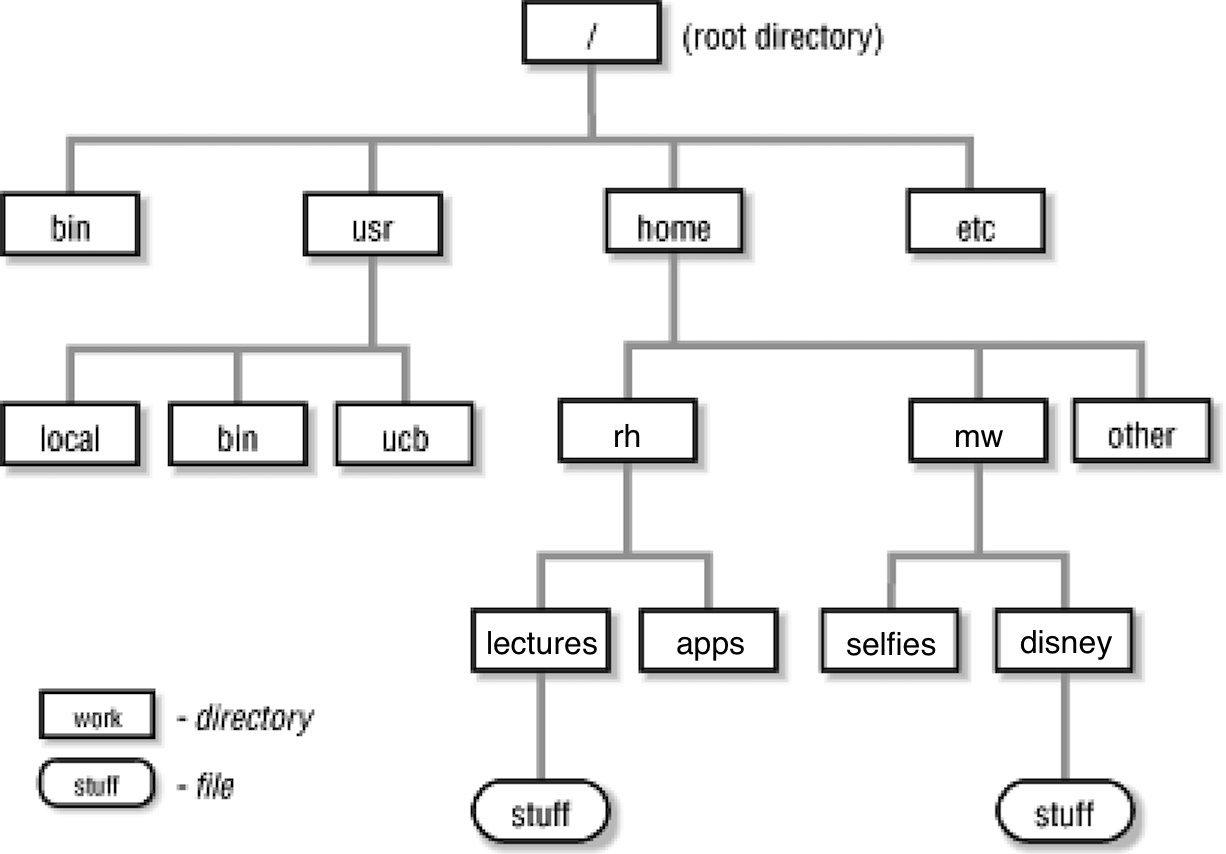
\includegraphics[height=8.5cm,keepaspectratio]{FS}
\end{frame}


\begin{frame}[fragile]\frametitle{Drives}
\begin{itemize}
\item On Unix, the file system has a unique \textbf{root directory} called \lstinline!/!
\begin{itemize}
    \item Every other directory is a child of it, or a child of a child, etc.
\end{itemize}
\bigskip
\item On Windows, every \textbf{drive} has its own root directory
\begin{itemize}
    \item So \lstinline!C:\home\rh\notes.txt! is different from \lstinline!J:\home\rh\notes.txt!
\end{itemize}
\end{itemize}
\end{frame}


\begin{frame}[fragile]\frametitle{Paths}
A \textbf{path} is a description of how to find something in a file system
\begin{itemize}
    \item An \textbf{absolute path} describes a location from the root directory down
\begin{itemize}
          \item Equivalent to a street address
          \item Always starts with "/"
          \item E.g., \lstinline{/home/rh} is my home directory, 
          \item and \lstinline{/home/rh/courses/prog1/UNIX1} is this file
\end{itemize}
    \item A \textbf{relative path} describes how to find something from some other location
\begin{itemize}
          \item Equivalent to saying, “Four blocks north of here, and seven blocks east”
\begin{itemize}
          \item E.g., from /home/rh, 
          \item the relative path to this file is courses/prog1/UNIX1
\end{itemize}
\end{itemize}
\end{itemize}
\end{frame}


\begin{frame}[fragile]\frametitle{Special Paths}
\begin{itemize}
\item Two special names:
\begin{itemize}
    \item "." means “the current working directory”
    \item ".." means “the directory immediately above this one
\begin{itemize}
          \item Also called the parent directory
\end{itemize}
\bigskip
 \item In /home/rh/courses/prog1/,
 \item .. is /home/rh/courses/
\end{itemize}
\end{itemize}
\end{frame}

\begin{frame}[fragile]\frametitle{Special Paths}
\begin{itemize}
\item Every program (including the shell) has a (current) working directory
\begin{itemize}
    \item “Where am I?”
    \item Relative paths are deciphered relative to this location
    \item Can change while a program is running
\end{itemize}
\end{itemize}
\end{frame}

\subsection{First  UNIX/Linux Commands}

\begin{frame}[fragile]\frametitle{pwd and ls}
\begin{itemize}
\item \textbf{pwd} prints (shows you) the current working directory
\end{itemize}
\begin{itemize}
\item \textbf{ls} lists the contents of that directory
\end{itemize}
\end{frame}

\begin{frame}[fragile]
\begin{block}{}
\begin{lstlisting}
-bash-4.1$ pwd
/u/w/maprh/accident reports
\end{lstlisting}
\end{block}
\end{frame}

\begin{frame}[fragile]
\begin{block}{}
\begin{lstlisting}
-bash-4.1$ ls
2_collision.pdf
747-300 Korean Air in Guam.pdf
A320_Bahrain.pdf
AAR0001.htm
accident summaries
ASN Aircraft accident description 31 JUL 1992 Thai Airways Airbus A_310 HS-TID_files
ASN Aircraft accident description 31 JUL 1992 Thai Airways Airbus A_310 HS-TID.htm
Bangkok
Cali
dasc98.ps
inhchart.pdf
-bash-4.1$ 
\end{lstlisting}
\end{block}
\end{frame}

\begin{frame}[fragile]\frametitle{More on ls}
What actually happens when I type ls is:
\begin{itemize}
    \item The operating system reads characters from the keyboard
    \item Passes them to the shell (because it's the currently active window on my desktop)
    \item The shell breaks the line of text it receives into words
    \item Looks for a program with the same name as the first word (i.e., the command to run)
    \item Runs that program
    \item Reads the program's output and sends it back to the operating system for display
\end{itemize}
\end{frame}

\begin{frame}[fragile]\frametitle{Flags}
\begin{itemize}
\item \textbf{Flags are options that you can add to commands}
\bigskip
\item E.g. can tell ls to produce more informative output by giving it some flags
\item By convention, flags start with "-", as in "-a" or "-l"
\end{itemize}
\end{frame}


\begin{frame}[fragile]\frametitle{Flags}
\begin{itemize}
\item For example: show directories with trailing slash
\end{itemize}
\begin{block}{}
\begin{lstlisting}
-bash-4.1$ ls -F
2_collision.pdf*
747-300 Korean Air in Guam.pdf*
A320_Bahrain.pdf*
AAR0001.htm*
accident summaries/
ASN Aircraft accident description 31 JUL 1992 Thai Airways Airbus A_310 HS-TID_files/
ASN Aircraft accident description 31 JUL 1992 Thai Airways Airbus A_310 HS-TID.htm*
Bangkok/
Cali/
\end{lstlisting}
\end{block}
\begin{itemize}
\item -a: gives you all files starting, including those, which are normally hidden
\item -l: provides long listing format i.e. provides more information
\end{itemize}
\end{frame}

\begin{frame}[fragile]\frametitle{Finding your way}
\begin{itemize}
\item man pages: provide an overview of the functionality of a command.
\begin{itemize}
\item !man ls!
\end{itemize}
\end{itemize}
\begin{itemize}
\item apropos: provides all commands related to a certain topic
\begin{itemize}
\item !appropos(permissions)!
\end{itemize}
\end{itemize}
\begin{itemize}
\item !--help!: provides support for a specific command
\begin{itemize}
\item !ls --help!
\end{itemize}
\end{itemize}
\end{frame}


\begin{frame}[fragile]\frametitle{Manipulating Files and Directories}
\begin{itemize}
\item Ultimately, we will want to create, use and delete our own files/directories
\item in oder to do that, we will need additional Unix commands:
\begin{itemize}
\item mkdir - create a new directory
\item cd - change directory
\item cp - copy a file
\end{itemize}
\end{itemize}
\end{frame}

\begin{frame}[fragile]\frametitle{Manipulating Files and Directories}
Working through an example:
\begin{itemize}
\item create a new directory called temp
\end{itemize}
\begin{block}{}
\begin{lstlisting}
      mkdir temp
\end{lstlisting}
\end{block}
\begin{itemize}
 \item Note: no output
 \item The -v (“verbose”) flag tells mkdir to print a confirmation message
\end{itemize}
\end{frame}

\begin{frame}[fragile]\frametitle{Manipulating Files and Directories}
\begin{itemize}
\item Now go into that directory
\end{itemize}
\begin{block}{}
\begin{lstlisting}
      cd temp
\end{lstlisting}
\end{block}
\begin{itemize}
\item Changes the shell's notion of our current working directory
\end{itemize}
\begin{block}{}
\begin{lstlisting}
      pwd 
      /home/rh/programming1/temp
\end{lstlisting}
\end{block}
\end{frame}

\begin{frame}[fragile]\frametitle{Manipulating Files and Directories}
\begin{itemize}
\item No files there yet:
\end{itemize}
\begin{lstlisting}
      ls -a
\end{lstlisting}
\begin{lstlisting}
      . ..
\end{lstlisting}
\begin{itemize}
\item Use the editor of your choice (emacs,vim) to create a file called earth.txt with the following contents:
\end{itemize}
\fbox{\footnotesize{\texttt{\begin{tabular}{l}
Name: Earth\\
Period: 365.26 days\\
Inclination: 0.00\\
Eccentricity: 0.02\\
Object: Planet\\
\end{tabular}}}}

\end{frame}

\begin{frame}[fragile]\frametitle{Manipulating Files and Directories}
\begin{itemize}
\item The easiest way to create a similar file venus.txt is to copy the one we have
\end{itemize}
\begin{block}{}
\begin{lstlisting}
      cp earth.txt venus.txt

      ls -t
      venus.txt   earth.txt
\end{lstlisting}
\end{block}
\begin{itemize}      
    \item Note: the syntax of the cp command (make a copy of earth.txt called venus.txt)
    \item Note also: the -t option tells ls to list newest first (i.e. list in time order)
\end{itemize}	
\end{frame}

\begin{frame}[fragile]\frametitle{Manipulating Files and Directories}
\begin{itemize}
    \item Check the contents of the file using \lstinline!cat! (short for “concatenate”)
    \item prints the contents of a file to the screen
    \item You can also use \lstinline!more! or \lstinline!less!
\end{itemize}	
\begin{block}{}
\begin{lstlisting}
      cat venus.txt
\end{lstlisting}
\end{block}
\end{frame}

\begin{frame}[fragile]\frametitle{Manipulating Files and Directories}
\begin{itemize}
\item Edit the file as follows:
\end{itemize}
\fbox{\footnotesize{\texttt{\begin{tabular}{l}
Name: Venus\\
Period: 224.70 days\\
Inclination: 3.39\\
Eccentricity: 0.01\\
Object: Planet
\end{tabular}}}}
\bigskip
\begin{itemize}
\item Compare the sizes of the two files using \lstinline!wc! (for “word count”) 
\end{itemize}
\begin{block}{}
\begin{lstlisting}[linewidth=5cm]
wc earth.txt venus.txt

  4   9  69 earth.txt
  4   9  69 venus.txt
  8  18 138 total
\end{lstlisting}
\end{block}
\end{frame}

\begin{frame}[fragile]\frametitle{Manipulating Files and Directories}
\begin{itemize}
\item You can also compare the files using the \textbf{diff} command
\item diff prints details of the differences between the files
\end{itemize}
\begin{block}{}
\begin{lstlisting}[linewidth=5cm]
diff earth.txt venus.txt

1,4c1,4
< Name: Earth
< Period: 365.26 days
< Inclination: 0.00
< Eccentricity: 0.02
---
> Name: Venus
> Period: 224.70 days
> Inclination: 3.39
> Eccentricity: 0.01
\end{lstlisting}
\end{block}
\end{frame}


\begin{frame}[fragile]\frametitle{Manipulating Files and Directories}
\begin{itemize}
\item Unix/Linux does not care about filename extensions.
\item cp earth.txt earth.pdf! is valid 
\item though not a very sensible thing to do
\bigskip
\item we can rename earth.pdf using \lstinline!mv earth.pdf earth2.txt!

\end{itemize}
\end{frame}

\begin{frame}[fragile]\frametitle{Manipulating Files and Directories}
\begin{itemize}
\item Removing a file can be done using \textbf{rm}
\end{itemize}

\begin{block}{}
\begin{lstlisting}[linewidth=5cm]
rm earth2.txt
\end{lstlisting}
\end{block}
\bigskip
\begin{itemize}
\item A empty directory can be removed with \lstinline!rmdir! or \lstinline!rm -r! which recursively removed all files.
\end{itemize}
\end{frame}

\begin{frame}[fragile]\frametitle{Next Steps}
\begin{itemize}
\item A practical next step to work through the university pages on UNIX/Linux
\begin{itemize}
\item http://www.bath.ac.uk/bucs/tools/unix/basicunixcommands/
\end{itemize}
\item Since many of you have asked, it is also worth noting that the University maintains a page on how to access the campus machines from outside (e.g. from your own laptops)
\begin{itemize}
\item http://www.bath.ac.uk/bucs/networking/ssh.html
\end{itemize}
\item We will look at connecting to one computer from another in the next UNIX lecture
\item .... but, for now, using the applications recommended by the University is not a bad starting point
\item As always, help is available in the labs

\end{itemize}
\end{frame}


\end{document}
